\chapter{Tableaux et Graphiques}\label{ChTableauxGraphiques}


\vspace{5cm}

\begin{acquis}
\begin{itemize}
\item savoir lire un graphique;
\item savoir lire un tableau à double entrées.
\end{itemize}
\end{acquis}


\activites

\begin{activite}[Lire un tableau]

Julie désire se rendre à Davos. Elle consulte les horaires des trains au départ d'Yverdon :

\begin{center}
\renewcommand*\tabularxcolumn[1]{>{\centering\arraybackslash}m{#1}}
 \begin{ttableau}{\linewidth}{7}
 \hline
 &  \cellcolor{F3} Train \newline n$^\circ$ 6\,123 & \cellcolor{F3} Train \newline n$^\circ$ 7\,258 & \cellcolor{F3} Train \newline n$^\circ$ 8\,766 & \cellcolor{F3} Train \newline n$^\circ$ 8\,989 & \cellcolor{F3} Train \newline n$^\circ$ 56\,789 & \cellcolor{F3} Train \newline n$^\circ$ 78\,995 \\
 \hline \cellcolor{F2} Yverdon & \cellcolor{Gris1} & 15 h 32 min & 16 h 05 min & 17 h 09 min & 17 h 20 min & 18 h 24 min \\
 \hline \cellcolor{F2} Bienne & 14 h 09 min & 16 h 32 min & \cellcolor{Gris1} & 17 h 58 min & 18 h 10 min & \cellcolor{Gris1} \\
 \hline \cellcolor{F2} Zürich  & 14 h 35 min & \cellcolor{Gris1} & \cellcolor{Gris1} & 18 h 11 min & 18 h 24 min & 19 h 18 min \\
 \hline \cellcolor{F2} Landquart & 14 h 58 min & \cellcolor{Gris1} & 17 h 32 min & \cellcolor{Gris1} & 18 h 47 min & \cellcolor{Gris1} \\
 \hline \cellcolor{F2} Davos & \cellcolor{Gris1} & 19 h 32 min & 20 h 15 min & 21 h 11 min & 21 h 32 min & 22 h 15 min \\
 \hline
 \end{ttableau}
 \end{center}

\vspace{1em}

\begin{partie}
Pourquoi certaines cases sont‑elles grisées ?
\end{partie}

\begin{partie}
Quel train est le plus rapide pour relier Yverdon à Davos ?
\end{partie}

\begin{partie}
En faisant une partie du trajet en voiture, Julie n'a passé que trois heures en train pour aller à Davos. De quelle(s) ville(s) a‑t‑elle bien pu partir ?
\end{partie}

\end{activite}

%%%%%%%%%%%%%%%%%%%%%%%%%%%%%%%%%%%%%%%%%%%%%%%%%%%%%%%%%%%%%%%%%%%%%%%%%

\begin{activite}[Utiliser des graphiques et des tableaux]

Pour déterminer quelques distances de freinage d'un véhicule sur route sèche, on a effectué des mesures à différentes vitesses, illustrées par le graphique ci-dessous :
\begin{center} 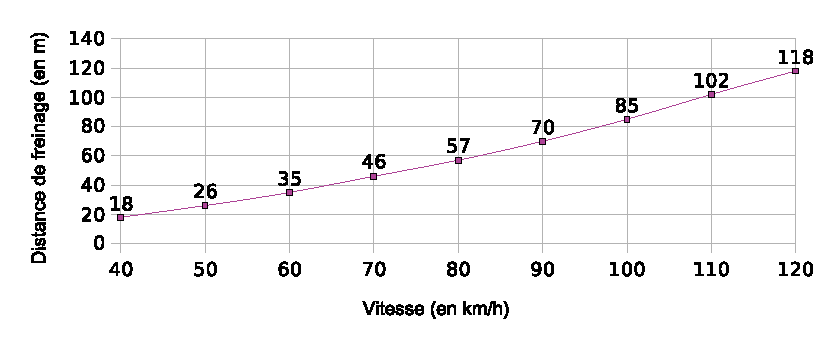
\includegraphics[width=14cm]{graph_freinage} \end{center}

\begin{partie}
Recopie et complète le tableau en utilisant le graphique :
\begin{center}
 \renewcommand*\tabularxcolumn[1]{>{\centering\arraybackslash}m{#1}}
 \begin{Ctableau}{\linewidth}{7}{c}
 \hline
 Vitesse (en km/h) & 50 & 70 & & & 110 & 120 \\\hline
 Distance de freinage (en m) & & & 70 & 85 & & \\\hline
  \end{Ctableau}
 \end{center}
\end{partie}

\vspace{1em}

\begin{partie}
Sur route mouillée, cette distance de freinage est deux fois plus grande que sur route sèche à vitesse égale.

Recopie et complète le tableau à double entrée suivant :
\begin{center}
 \renewcommand*\tabularxcolumn[1]{>{\centering\arraybackslash}m{#1}}
 \begin{Ctableau}{\linewidth}{4}{c}
 \hline
 Vitesse (en km/h) & 70 & & \\\hline
 Distance de freinage sur route sèche (en m) & & 35 &  \\\hline
 Distance de freinage sur route mouillée (en m) & & & 140 \\\hline
  \end{Ctableau}
 \end{center}
\end{partie}

\vspace{1em}

\begin{partie}
Aujourd'hui il pleut, et Joël part pour un petit tour de voiture en ville.

S'il doit s'arrêter pour éviter un obstacle, combien de mètres fera‑t‑il au maximum avant l'arrêt de son véhicule, s'il roule à la vitesse de 50 km/h.
\end{partie}

\end{activite}

%%%%%%%%%%%%%%%%%%%%%%%%%%%%%%%%%%%%%%%%%%%%%%%%%%%%%%%%%%%%%%%%%%%%%%%%%

\begin{activite}[Regrouper des données dans un tableau]

Dans un village, on a demandé aux familles le nombre d'enfants qu'elles avaient à charge. Le tableau ci‑dessous donne les réponses de chaque foyer.
\begin{center} 2 ; 3 ; 0 ; 1 ; 0 ; 1 ; 4 ; 2 ; 2 ; 0 ; 1 ; 6 ; 2 ; 3 ; 0 ; 7 ; 1 ; 0 ; 3 ; 2 ; 1 ; 3 ; 1 ; 3 ; 1 ; 1 ; 0 ; 7 ; 2 \end{center}

\begin{partie}
Recopie et complète le tableau suivant :
\begin{center}
\begin{tabularx}{\linewidth}{|c|*{10}{>{\centering \arraybackslash}X|}}
\hline \cellcolor{J1} Nombre d'enfants & 0 & 1 & 2 & 3 & 4 & 5 & 6 & 7 & Total \\
\hline \cellcolor{J2} Nombre de familles & & & & & & & & & \\
\hline
\end{tabularx} \\
\end{center}
\end{partie}

\vspace{1em}

\begin{partie}
Combien de familles ont quatre enfants ? \textbf{Moins de} trois enfants ? Combien de familles ont \textbf{exactement} quatre enfants ?
\end{partie}

\begin{partie}
Combien de familles ont \textbf{au moins} deux enfants ? \textbf{Plus de} quatre enfants ? \textbf{Au plus} quatre enfants ?
\end{partie}

\end{activite}

%%%%%%%%%%%%%%%%%%%%%%%%%%%%%%%%%%%%%%%%%%%%%%%%%%%%%%%%%%%%%%%%%%%%%%%%%

\begin{activite}[Utiliser un tableur]

\begin{partie}[À la cantine]
L'intendante du collège \emph{Rivegauche} a relevé le nombre de fois où chaque élève demi‑pensionnaire de sixième mange à la cantine durant la semaine et elle a reporté les résultats dans un tableau.
\begin{enumerate}
 \item Recopie son tableau dans une feuille de calcul en suivant ce modèle :
 \begin{center}
\begin{tabularx}{\linewidth}{|c|c|X|X|X|X|X|X|}
\hline \rowcolor{Gris1} & A & B & C & D & E & F & G \\
\hline \cellcolor{Gris1} 1 & & 1 jour & 2 jours & 3 jours & 4 jours & 5 jours & \\
\hline \cellcolor{Gris1} 2 & \cellcolor{G3} Nombre d'élèves & \cellcolor{J1} 20 & 33 & 21 & 47 & 37 & \cellcolor{B3} \\
\hline
\end{tabularx} \\
\end{center}
\vspace{.5em}
 \item Comment pourrais-tu nommer la cellule orange ? La verte ? La rose ?
 \item Combien de repas ont été servis à la cantine durant la semaine ? \label{TabsGraphsActi}
 \item Le tableur est capable de reproduire ce calcul si l'on saisit une formule dans la cellule $G2$. Une formule commence toujours par le signe «\,=\,». 
  \begin{itemize}
   \item Place le curseur dans la cellule $G2$ puis saisis la formule : « $= B2 + C2 + D2 + E2 + F2$ ». Appuie sur la touche «\,Entrée\,» du clavier. 
   \item Obtiens‑tu le même résultat qu'à la question \ref{TabsGraphsActi} ?
   \end{itemize}
 \item C'est le repas de Noël au collège ! Marc, Sonia et Sam, trois externes, désirent rejoindre leurs amis pour l'occasion. Modifie une cellule pour faire apparaître le changement d'effectif. Que remarques‑tu pour la cellule $G2$ ?
 \end{enumerate}
\end{partie}

\begin{partie}[Que de livres !]
En novembre 2009, l'imprimerie Volléro produit 2\,100 livres. Le directeur décide d'augmenter la production de 220 livres chaque mois dès le mois de décembre.
\begin{enumerate}
 \item Recopie le tableau suivant dans une feuille de calcul :
 \begin{center}
\begin{tabularx}{1.05\linewidth}{|c|*{6}{>{\centering \arraybackslash}X|}}
\hline \rowcolor{Gris1} & A & B & C & D & E \\
\hline \cellcolor{Gris1} 1 & \cellcolor{G3} Mois & \small{Novembre} 2009 & \small{Décembre} 2009 & \small{Janvier} 2010 & \small{Février} 2010
 \\
\hline \cellcolor{Gris1} 2 & \cellcolor{G2} Nombre de livres & 2\,100 & & & \\
\hline
\end{tabularx} \\
\end{center}
\vspace{0.5cm}         
 \item Saisis les formules permettant de compléter le tableau.
 \item Comment ferais‑tu pour calculer le nombre de livres produits en mars 2010 ?
 
Le tableur peut reproduire cette méthode en saisissant une formule dans la cellule $F2$.
 \item Place le curseur dans la cellule $F2$ et saisis la formule : « $= E2 + 220$ ». Comment comprends‑tu cette formule ?
 \item Quelle serait la formule à saisir en $G2$ pour calculer le nombre de livres produits en avril 2010 ? \label{Tabs&Graphs_acti2}
 \item Copie le contenu de la cellule $F2$ et colle‑le dans la cellule $G2$. Tu peux voir le résultat sur la ligne située au-dessus de ta feuille de calcul. Que s'est‑il passé ?
\begin{center} 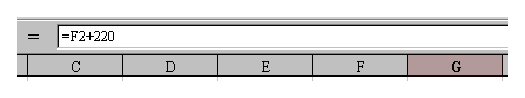
\includegraphics[width=11.2cm]{feuille_calcul} \end{center}
 \item Le directeur aimerait savoir quand (mois et année) son usine produira plus de 8\,000 livres par mois. En répétant plusieurs fois la méthode de la question \ref{Tabs&Graphs_acti2}, réponds à la question du directeur.
 \end{enumerate}
\end{partie}


\end{activite}

%%%%%%%%%%%%%%%%%%%%%%%%%%%%%%%%%%%%%%%%%%%%%%%%%%%%%%%%%%%%%%%%%%%%%%%%%

\cours
%\section{Une section}

% remarque : pour qu'un mot se retrouve dans le lexique : \MotDefinition{asymptote horizontale}{} 

Bla bla

\begin{aconnaitre}
Bla bla
\end{aconnaitre}



\exercicesbase
\begin{colonne*exercice}

\serie{Lecture de tableaux}

\begin{exercice}[Promenons‑nous dans les bois]
Dans le bois, j'ai fait le relevé suivant : trois‑cent‑vingt arbres sont des chênes, cent‑vingt arbres sont des hêtres et j'ai compté quarante sapins. Recopie et complète le tableau :
 \begin{center}
 \renewcommand*\tabularxcolumn[1]{>{\centering\arraybackslash}m{#1}}
 \begin{ttableau}{\linewidth}{5}
  \hline
  & \cellcolor{H2} Chênes & \cellcolor{H2} Hêtres & \cellcolor{H2} Sapins & \cellcolor{H2} Total \\\hline
  \rowcolor{H2} Nombre & & & & \\\hline
  \end{ttableau}
\end{center}
\end{exercice}


\begin{exercice}[Regrouper des notes]
Voici les points obtenus dans un test de mathématiques :

12 ; 10 ; 11 ; 12 ; 14 ; 19 ; 10 ; 15 ; 20 ; 09 ; 18 ; 14 ; 12 ; 11 ; 12 ; 11 ; 11 ; 08 ; 10 ; 14.
\begin{enumerate}
 \item Combien d'élèves ont obtenu 10 points ou moins ?
 \item Combien d'élèves ont obtenu entre 11 et 15 points ?
 \item Combien d'élèves ont obtenu 16 points ou plus ?
 \end{enumerate}
\end{exercice}


\begin{exercice}[Facture]
 Voici un extrait d'une facture téléphonique :
 \begin{center}
 \begin{tabularx}{\linewidth}{|l|X|X|X|}
  \hline
  & \cellcolor{J1} Prix HT en CHF & \cellcolor{J1} TVA  en CHF & \cellcolor{J1} Prix TTC en CHF \\\hline
 \cellcolor{J1} Abonnement & \cellcolor{J3} 29,26 & \cellcolor{J3} 5,73 & \cellcolor{J3} A  \\\hline
 \cellcolor{J1} Consommation &  \cellcolor{J3} 7,98 &  \cellcolor{J3} B &  \cellcolor{J3} 9,54  \\\hline
  \end{tabularx}
 \end{center}
Le montant TTC (toutes taxes comprises) s'obtient en additionnant la TVA au montant HT (hors taxes).
\begin{enumerate}
 \item Quelles sont les valeurs de $A$ et $B$ ? Justifie.
 \item Donne un ordre de grandeur du montant total nécessaire pour régler cette facture.
 \end{enumerate}
\end{exercice}


\begin{exercice}[Horaires]
Voici un extrait d'horaires du RER :
 \begin{center}
 \begin{tabularx}{\linewidth}{|c|X|X|X|X|X|}
  \hline
   & \cellcolor{A3} \quad \rotatebox{90}{RER 1} & \cellcolor{A3} \quad \rotatebox{90}{RER 2} & \cellcolor{A3} \quad \rotatebox{90}{RER 3} & \cellcolor{A3} \quad \rotatebox{90}{RER 4} & \cellcolor{A3} \quad \rotatebox{90}{RER 5} \\\hline
  \rowcolor{A4} Coppet & 7.22 & 8.12 & 9.10 & 18.45 & 20.14 \\\hline
  \rowcolor{A3} Mies & 7.32 & 8.20 & 9.18 & & 20.23 \\\hline
  \rowcolor{A4} Versoix & 7.40 & 8.27 & 9.25 & 18.59 & 20.30 \\\hline
  \rowcolor{A3} Genève & 7.57 & 8.41 & 9.45 & & 20.44 \\\hline
  \rowcolor{A4} Vernier & 8.07 & 8.50 & 9.56 & & 20.53 \\\hline
  \rowcolor{A3} Russin & 8.20 & 9.03 & 10.09 & & 21.06 \\\hline
  \rowcolor{A4} La Plaine & & 9.22 & & & \\\hline
  \rowcolor{A3} Bellegarde & 8.44 & 9.30 & 10.32 & 19.56 & 21.29 \\\hline
  \end{tabularx}
\end{center}
\begin{enumerate}
 \item Que signifient les cases vides du tableau ?
 \item Malika veut arriver à Bellegarde avant 10 h. Elle part de Vernier. Quel(s) train(s) peut‑elle choisir ?
 \item Finalement, elle prend le train de 8 h 50. Quelle est la durée du trajet ?
 \item Sébastien part de Coppet après 18 h pour aller à Bellegarde. Il décide de prendre le train le plus rapide. Quel train va‑t‑il choisir ?
 \end{enumerate}
\end{exercice}

%%%%%%%%%%%%%%%%%%%%%%%%%%%%%%%%%%%%%%%%%%%%%%%%%%%%%%%%%%%%%%%%%%%%%%%%%%%%%%

\serie{Lecture de graphiques}

\begin{exercice}[Températures]
Températures relevées un jour de juillet 2008 à Sion :
\begin{center} 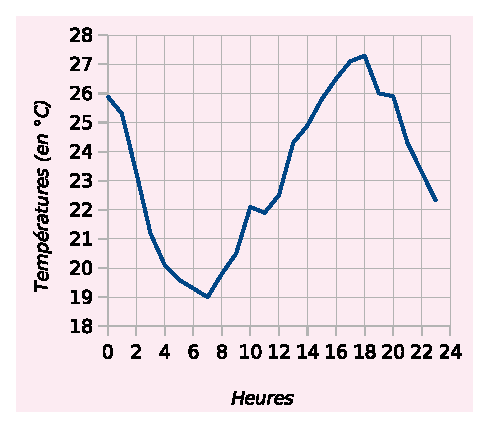
\includegraphics[width=8cm]{temperatures} \end{center}
\begin{enumerate}
 \item Quelle température faisait‑il à 4 h ?
 \item Quand a‑t‑il fait $25^\circ$C ?
 \item À quelle période de la journée la température est‑elle la plus élevée ? La plus basse ?
 \end{enumerate}
\end{exercice}

%%%%%%%%%%%%%%%%%%%%%%%%%%%%%%%%%%%%%%%%%%%%%%%%%%%%%%%%%%%%%%%%%%%%%%%%%%%%%%

\serie{Interprétation}

\begin{exercice}[Langue vivante]
Un collège compte 240 élèves. Les élèves sont, soit demi‑pensionnaires (D.P.), soit externes. Chacun de ces élèves étudie une 2\up{ème} langue au choix : anglais, allemand ou espagnol. \\[0.5em]
Quelles sont les valeurs de $A$, $B$, $C$, $D$, $E$, $F$, $G$ ? Justifie.
 \begin{center}
 \begin{tabular}{|c|c|c|c|c|}
  \hline
  & \cellcolor{A3} \small{Anglais} & \cellcolor{A3} \small{Allemand} & \cellcolor{A3} \small{Espagnol} & \cellcolor{A3} \small{Total} \\\hline
  \rowcolor{A4} \small{D.P.} & $A$ & 40 & 60 & 130 \\\hline
  \rowcolor{A3} \small{Externes} & $B$ & $C$ & $D$ & $E$ \\\hline
  \rowcolor{A4} \small{Total} & 66 & 72 & $F$ & $G$ \\\hline
  \end{tabular}
\end{center}
\end{exercice}


\begin{exercice}[Une entreprise]
Le graphique suivant illustre les ventes (en milliers) d'une fabrique de jouets.
\begin{center} 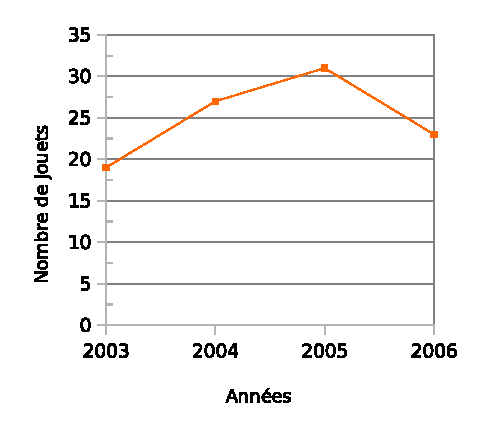
\includegraphics[width=8cm]{graph_entreprise} \end{center}
\begin{enumerate}
 \item En quelle année cette entreprise a‑t‑elle réalisé ses meilleures ventes ?
 \item Décris l'évolution du nombre de ventes de jouets de 2003 à 2006.
 \item Recopie et complète le tableau :
 \begin{center}
  \renewcommand*\tabularxcolumn[1]{>{\centering\arraybackslash}m{#1}}
  \begin{ttableau}{\linewidth}{5}
   \hline
   \rowcolor{J1} Année & 2003 & & & \\\hline
   \rowcolor{J2} \small{Nombre de jouets} & & 27 000 & & \\\hline
  \end{ttableau}
 \end{center}
 \item Combien de jouets ont été vendus de 2003 à 2006 ?
\end{enumerate}
\end{exercice}


\begin{exercice}[Sécurité routière]
Le tableau ci‑dessous donne la répartition, par tranche d'âge, du nombre des victimes dans des accidents dus à l'alcool, en 2007 :
 \begin{center}
  \renewcommand*\tabularxcolumn[1]{>{\centering\arraybackslash}m{#1}}
  \begin{ttableau}{\linewidth}{2}
   \hline
   \rowcolor{C2} Tranches d'âge & Nombre de tués \\\hline
   \cellcolor{U1} 0 ‑ 17 ans & 22 \\\hline
   \cellcolor{U1} 18 ‑ 24 ans & 228 \\\hline
      \cellcolor{U1} 25 ‑ 44 ans & \\\hline
   \cellcolor{U1} 45 ‑ 64 ans & 172 \\\hline
   \cellcolor{U1} 65 ans et plus & 39 \\\hline
   \cellcolor{U1} Âge inconnu & 3 \\\hline
  \end{ttableau}
 \end{center}
\begin{enumerate} 
 \item Le nombre total de tués dans des accidents dus à l'alcool en 2007 est de 966. Recopie et complète le tableau.
 \item Quelle est la tranche d'âge la plus touchée ?
 \end{enumerate}
\end{exercice}



\begin{exercice}[En géométrie]
\begin{center} 
\includegraphics[width=6cm]{tableau_geometrie} \end{center}
\begin{enumerate}
 \item Recopie et complète le tableau par $\in$ ou $\notin$ : \\[0.3em]
  \begin{center}
 \begin{tabularx}{\linewidth}{|c|X|X|X|}
  \hline
   & \cellcolor{F3} Droite $d$ & \cellcolor{F3} Droite $d'$ & \cellcolor{F3} Cercle $\mathcal{C}$ \\\hline
  \cellcolor{H3} A & & & \\\hline
  \cellcolor{H3} B & & & \\\hline
  \cellcolor{H3} C & & & \\\hline
  \cellcolor{H3} D & & & \\\hline
  \cellcolor{H3} E & & & \\\hline
  \end{tabularx}
\end{center}
\vspace{0.5cm}
 \item Construis une figure correspondant au tableau ci‑dessous : \\[0.3em]
  \begin{center}
 \begin{tabularx}{\linewidth}{|c|X|X|X|}
  \hline
   & \cellcolor{F3} Cercle $\mathcal{C}_1$ & \cellcolor{F3} Droite $d$ & \cellcolor{F3} Cercle $\mathcal{C}_2$ \\\hline
  \cellcolor{H3} A & $\in$ & $\notin$ & $\in$ \\\hline
  \cellcolor{H3} B & $\notin$ & $\in$ & $\notin$ \\\hline
  \cellcolor{H3} C & $\notin$ & $\notin$ & $\in$ \\\hline
  \cellcolor{H3} D & $\in$ & $\in$ & $\in$ \\\hline
  \cellcolor{H3} E & $\notin$ & $\in$ & $\notin$ \\\hline
  \end{tabularx}
\end{center}
 \end{enumerate}
\end{exercice}
\end{colonne*exercice}


\exercicesappr
\begin{colonne*exercice}
\begin{exercice}[Dépenses culturelles et de loisirs]
Voici un texte analysant l'évolution de certaines dépenses culturelles et de loisirs des Suisses au cours des vingt dernières années. \\[0.5em]
« \emph{Les Suisses ont plus de temps libre, ce qui explique que leurs dépenses pour les loisirs (cinéma, concerts) augmentent régulièrement. Les dépenses en multimédia ont explosé au début des années 90 et sont constantes depuis. Nombreux sont ceux qui consultent les informations sur Internet et se désintéressent de la lecture des journaux...}

\emph{De même, les ventes de disques ou pellicules photo sont en diminution constante (cette catégorie est à présent la moins importante), ce qui s'explique par le « boum » de la photo numérique ou du téléchargement musical. Après avoir diminué, les ventes de téléviseurs ont tendance à redémarrer, grâce à la baisse des prix des écrans plats.} » \\[0.5em]
Le tableau suivant correspond au commentaire ci‑dessus. Les données sont données en pour cent.
 \begin{center}
  \renewcommand*\tabularxcolumn[1]{>{\centering\arraybackslash}m{#1}}
  \begin{ttableau}{\linewidth}{4}
   \hline
   \rowcolor{A2} \textbf{Dépense} & \textbf{1990} & \textbf{2000} & \textbf{2007} \\\hline
   \cellcolor{A2} \textbf{1} & 14,7 & 10,8 & 11,5 \\\hline
   \cellcolor{A2} \textbf{2} & 1,9 & 7,7 & 7,8 \\\hline
   \cellcolor{A2} \textbf{3} & 5,9 & 5,5 & 3,5 \\\hline
   \cellcolor{A2} \textbf{4} & 14,1 & 16,4 & 18,2 \\\hline
   \cellcolor{A2} \textbf{5} & 20,2 & 15,8 & 13,4 \\\hline
  \end{ttableau}
 \end{center}
\begin{enumerate}
 \item Indique à quelle catégorie de dépenses correspond chaque ligne du tableau, parmi les suivantes :
 \begin{itemize}
  \item Spectacles, cinéma et voyage ;
  \item Informatique ;
  \item Presse, livres et papeterie ;
  \item TV, Hi‑fi, vidéo ;
  \item Disques, cassettes, pellicules photo.
  \end{itemize}
 \item Calcule le total de chaque colonne du tableau. Comment expliques‑tu tes résultats ?
 \end{enumerate}
\end{exercice}



%%%%%%%%%%%%%%%%%%%%%%%%%%%%%%%%%%%
%%%%%%%%%%%%%%%%%%%%%%%%%%%%%%%%%%%
%MiseEnPage
%%%%%%%%%%%%%%%%%%%%%%%%%%%%%%%%%%%
\columnbreak
%%%%%%%%%%%%%%%%%%%%%%%%%%%%%%%%%%%
%%%%%%%%%%%%%%%%%%%%%%%%%%%%%%%%%%%

\begin{exercice}[Énergies renouvelables : prévisions]
Le tableau suivant indique le nombre d'emplois prévus dans différents secteurs des énergies renouvelables (\textcolor{PartieGeometrie}{en milliers d’emplois}).

Source : \emph{Rapport MITRE (2003) commandité par la Commission Européenne.}
 \begin{center}
 \begin{tabularx}{1.03\linewidth}{|c|X|X|X|X|X|X|X|X|X|}
  \hline
   & \cellcolor{H1} \rotatebox{90}{Biomasse} & \cellcolor{H1} \rotatebox{90}{Biocarburants} & \cellcolor{H1} \rotatebox{90}{Éolien} & \cellcolor{H1} \rotatebox{90}{Biogaz} & \cellcolor{H1} \rotatebox{90}{Solaire Thermique} & \cellcolor{H1} \rotatebox{90}{Photovoltaïque} & \cellcolor{H1} \rotatebox{90}{Micro-hydraulique\phantom{.}} & \cellcolor{H1} \rotatebox{90}{Pompes à chaleur} & \cellcolor{H1} \rotatebox{90}{\textbf{Total}} \\\hline
  \cellcolor{C2} Emplois en 2004 & \rotatebox{90}{25} & \rotatebox{90}{4.2\phantom{.}} & \rotatebox{90}{2} & \rotatebox{90}{0.1} & \rotatebox{90}{1} & \rotatebox{90}{1} & \rotatebox{90}{2.4} & \rotatebox{90}{3.2} & \\\hline
  \cellcolor{C2} Emplois en 2010 & \rotatebox{90}{45} & \rotatebox{90}{20} & & \rotatebox{90}{2} & \rotatebox{90}{10.5} & \rotatebox{90}{3.5} & \rotatebox{90}{2.4} & \rotatebox{90}{10} & \rotatebox{90}{115.4} \\\hline
  \end{tabularx}
\end{center}
\begin{enumerate}
 \item Combien d'emplois prévoit ce rapport pour la filière éolienne en 2010 ?
 \item Est‑il vrai que le nombre d'emplois dans le secteur des pompes à chaleur aura quasiment triplé entre 2004 et 2010 ?
 \item Combien d'emplois auront été créés entre 2004 et 2010 si ces prévisions se confirment ?
 \end{enumerate}
\end{exercice}

%%%%%%%%%%%%%%%%%%%%%%%%%%%%%%%%%%%
%%%%%%%%%%%%%%%%%%%%%%%%%%%%%%%%%%%
%MiseEnPage
%%%%%%%%%%%%%%%%%%%%%%%%%%%%%%%%%%%
\newpage
%%%%%%%%%%%%%%%%%%%%%%%%%%%%%%%%%%%
%%%%%%%%%%%%%%%%%%%%%%%%%%%%%%%%%%%

\begin{exercice}[Ça chauffe !]
Afin de surveiller ses dépenses de chauffage cet hiver, M. Frigo a décidé de contrôler sa consommation de mazout. Les graphiques suivants représentent la quantité de fuel restant dans sa cuve, en fonction du temps. \\[1em]
\textbf{\textcolor{A2}{En fin d'année}}

M. Frigo a commencé ses relevés fin novembre :
\begin{center} 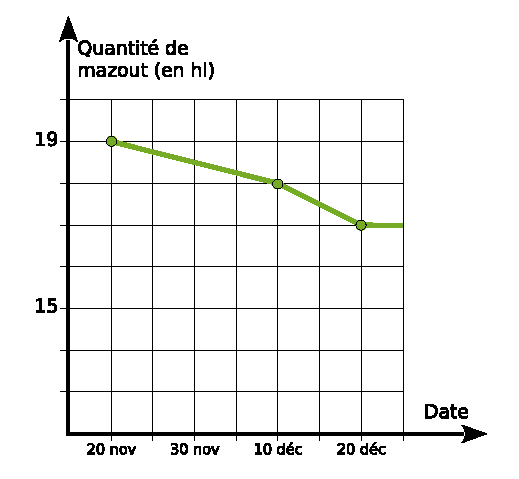
\includegraphics[width=8cm]{graph_frigo1} \end{center}

\begin{enumerate}
 \item Quelle quantité de mazout contenait sa cuve au 20 novembre ? 
 \item Quelle quantité de mazout a‑t‑il consommée du 20 novembre au 20 décembre ?
 \item Une vague de froid est survenue durant cette période \ldots Au vu du graphique, peux‑tu préciser quand ?
 \item Selon toi, M. Frigo a‑t‑il passé le jour de Noël à la maison ? Explique ta réponse. \\[1em]
 
 \textbf{\textcolor{A2}{Au début de l'année}}
 
\begin{center} 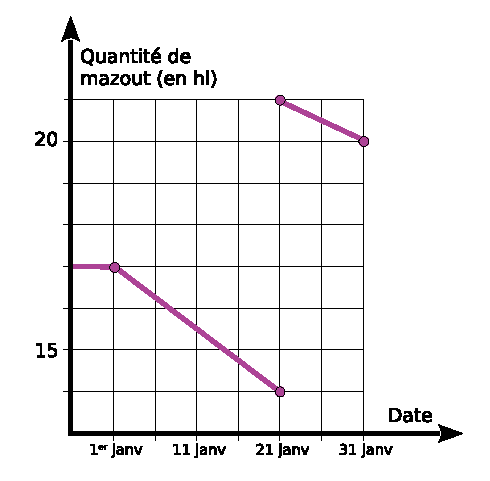
\includegraphics[width=8cm]{graph_frigo2} \end{center} 

 \item Quand M. Frigo a‑t‑il remis sa chaudière en route ?
 \item Que s'est‑il passé le 21 janvier ?
 \item Quelle quantité de mazout a‑t‑il consommée entre le 20 novembre et le 31 janvier ?
 \item Combien d'argent M. Frigo a‑t‑il dépensé durant cette période, sachant que le prix du litre de mazout était de 0,90 CHF ?
 \begin{center} 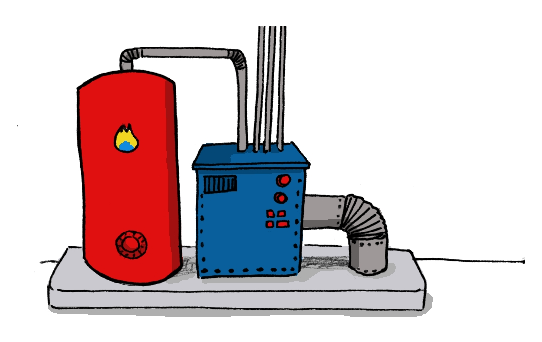
\includegraphics[width=4.5cm]{mazout} \end{center}
 \end{enumerate}
\end{exercice}




\end{colonne*exercice}

\connaissances

\QCMautoevaluation{Pour chaque question, plusieurs réponses sont
  proposées.  Déterminer celles qui sont correctes.}

\begin{QCM}
  \begin{GroupeQCM}
  \begin{minipage}[c]{0.44\linewidth}
  Le tableau ci‑contre donne le nombre d'ordinateurs possédés par les familles des élèves de sixième du collège Fontbruant. Il ne concerne que les trois premières questions.
   \end{minipage} \hfill%
   \begin{minipage}[c]{0.52\linewidth}
   \begin{center}
    \begin{tabularx}{\linewidth}{|c|X|X|X|X|c|}
    \hline
    Nombre d'ordinateurs & 0 & 1 & 2 & 3 & 4 et plus \\\hline
    Nombre d'élèves & 5 & 19 & 25 & 13 & 8 \\\hline
  \end{tabularx}
   \end{center}
    \end{minipage}\\[1em]
    
    \begin{exercice}
      à quelle(s) question(s) est‑il possible de répondre à l'aide du tableau ?
      \begin{ChoixQCM}{4}
      \item Combien d'élèves de sixième ont un (et un seul) ordinateur ?
      \item Combien d'élèves ont plus de quatre ordinateurs ?
      \item Combien de ces familles sont équipées d'ordinateurs ?
      \item Combien y a‑t‑il d'élèves dans le collège ?
      \end{ChoixQCM}
\begin{corrige}
     \reponseQCM{abc} 
   \end{corrige}
    \end{exercice}
    
    
    \begin{exercice}
      D'après le tableau, on peut dire que \ldots
      \begin{ChoixQCM}{4}
      \item 24 élèves ont au moins deux ordinateurs
      \item À eux tous, ils ont 145 ordinateurs
      \item 21 élèves ont plus de deux ordinateurs
      \item Il y a 70 élèves en sixième
      \end{ChoixQCM}
\begin{corrige}
     \reponseQCM{d}
   \end{corrige}
    \end{exercice}
    
    
    \begin{exercice}
      Si les ordinateurs étaient répartis équitablement, les élèves auraient environ \ldots
      \begin{ChoixQCM}{4}
      \item 1 ordinateur chacun
      \item 2 ordinateurs chacun 
      \item 3 ordinateurs chacun
      \item 4 ordinateurs chacun
      \end{ChoixQCM}
\begin{corrige}
     \reponseQCM{b}
   \end{corrige}
    \end{exercice}
    
    
    \begin{exercice}
      \begin{center} 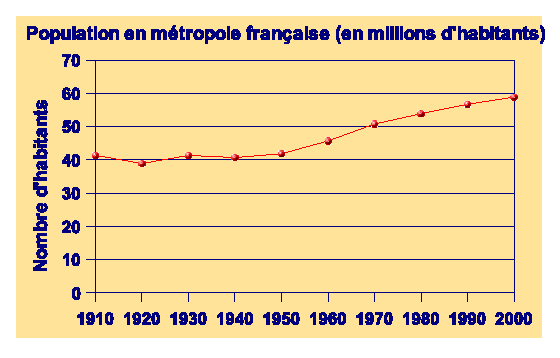
\includegraphics[width=6cm]{agmentation_popul} \end{center}
      \begin{ChoixQCM}{4}
      \item La population augmente depuis 1940
      \item La population a atteint 50 millions d'habitants en 1960
      \item Le nombre d'habitants était quasiment le même en 1910 et 1930
      \item Le nombre d'habitants est, durant cette période, resté inférieur à 60 millions
      \end{ChoixQCM}
\begin{corrige}
     \reponseQCM{acd}
   \end{corrige}
    \end{exercice}
 
 
    \begin{exercice}
    Origine des véhicules situés sur un parking : \hspace{1em} 
    \begin{minipage}[c]{4cm}
    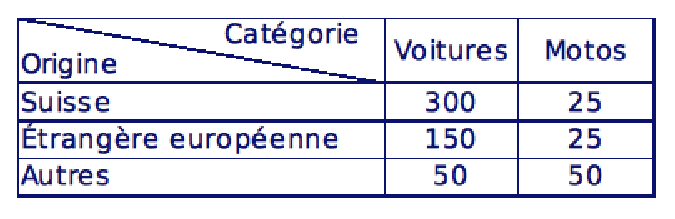
\includegraphics[width=\textwidth]{parking_auto}
    \end{minipage}
%      \begin{center} 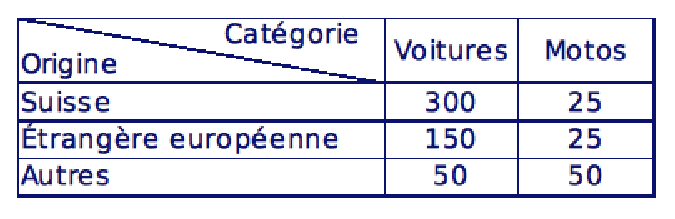
\includegraphics[width=4.5cm]{parking_auto} \end{center}
      \begin{ChoixQCM}{4}
      \item 500 véhicules Suisses sont stationnés sur le parking
      \item La moitié des véhicules sont de nationalité étrangère
      \item Les voitures sont 5 fois plus nombreuses que les motos
      \item 600 personnes ont garé leur véhicule sur le parking
      \end{ChoixQCM}
\begin{corrige}
     \reponseQCM{cd}
   \end{corrige}
    \end{exercice}
    

\end{GroupeQCM}
\end{QCM}

  


\TravauxPratiques % pour nous "travailler en groupe"

\begin{TP}[Enquête]

\partie{En petits groupes}

\begin{enumerate}
 \item Rédigez un questionnaire commun à la classe pour mieux connaître les élèves (« garçon ou fille ? », «nombre de frères et sœurs ? », « activité favorite », « temps accordé aux devoirs ? », etc.) puis répondez‑y.
 \item Résumez vos réponses dans des tableaux et des graphiques.
 \item Présentez ensuite les résultats du groupe au reste de la classe.
 \end{enumerate}
 
\partie{Voyons plus grand !}

\begin{enumerate}
\setcounter{enumi}{3}
 \item À l'aide des réponses des autres groupes, construis des tableaux et des graphiques illustrant le profil de la classe. \\[1em]
Y a‑t‑il un groupe dont les réponses sont proches de celles de l'ensemble de la classe ?
 \end{enumerate}
 
 
%%%%%%%%%%%%%%%%%%%%%%%%%%%%%%%%%%%%
%%%%%%%%%%%%%%%%%%%%%%%%%%%%%%%%%%%
%MiseEnPage
%%%%%%%%%%%%%%%%%%%%%%%%%%%%%%%%%%%
\vfill
%%%%%%%%%%%%%%%%%%%%%%%%%%%%%%%%%%%
%%%%%%%%%%%%%%%%%%%%%%%%%%%%%%%%%%%
 
\end{TP}



\pagebreak

\recreation
\begin{enigme}[Bon pour la santé ?]

Dans une publicité pour un yaourt à boire VITALAIT, on peut lire :

 « VITALAIT est la boisson qui vous aide à renforcer vos défenses naturelles. ».


\begin{minipage}[c]{0.31\linewidth} 
 \begin{center} 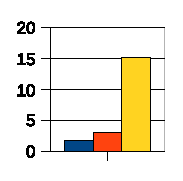
\includegraphics[width=2.4cm]{graph_VITALAIT} \end{center}
 \begin{center} \small{répartition pour 100g de VITALAIT} \end{center}
 \end{minipage} \hfill%
 \begin{minipage}[c]{0.31\linewidth} 
 \begin{center} 
\includegraphics[width=2.4cm]{apport_nutrition} \end{center}
 \end{minipage} \hfill%
 \begin{minipage}[c]{0.31\linewidth}
 \begin{center} 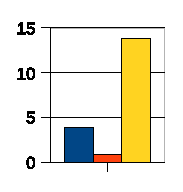
\includegraphics[width=2.4cm]{graph_yaourt} \end{center}
 \begin{center} \small{répartition pour 100g de yaourt sucré} \end{center}
  \end{minipage} \\

\begin{enumerate}
 \item Cherche les définitions des glucides, lipides et protides.
 \item Penses‑tu que le slogan publicitaire du produit « VITALAIT » est pertinent ? Justifie.
 \end{enumerate}

\begin{minipage}[c]{0.2\linewidth}   
 
\includegraphics[width=2.4cm]{VITALAITvsYAOURT}
 \end{minipage}
 \begin{minipage}[c]{0.38\linewidth} 
 \textbf{\textcolor{C1}{Information}} : il y a autant de bactéries (plus de 10 milliards) dans un VITALAIT que dans un yaourt ordinaire.
 \end{minipage} \\
\end{enigme} 



